\documentclass[11pt, twocolumn]{article}
\pagestyle{plain}
\usepackage{geometry}
\usepackage{graphicx}
\usepackage{float}
\geometry{
    body={6.5in,9.5in},
    left= 1.0in,
    top = 0.5in}

\begin{document}
\title{{\bf Automatic Action Discovery in Psychological videos}\\ \vspace{10pt}
			 { \normalsize {Diwakar Chauhan \\ Guide : Amitabha Mukerjee \\ \{diwakarc, amit\}@cse.iitk.ac.in}}}
%\date{\today}
\maketitle
%\newpage

\section*{Abstract :}
Activity recognition is an essential part of several applications. Robotics, smart homes, monitoring are the major areas which involve activity recognition. Lot's of work has been done on computer vision based activity recognition. It involves tracking the agents and understanding the behaviour of agents and their interaction. One more aspect of activity recognition is to assign linguistic to the activities. This process is very closely  related to human learning process. An infant learns the nouns in first place than verbs. The reason behind this may be that verbs therefore activities require more information and information of different kind. Naigles(1990)\cite{naigles} demonstrated that while learning meaning of verbs, infants use the syntactic information. She proved that given a illegal verbs in a sentence the children use the syntax to guess the meaning of the verb. \\
\hspace*{10pt} However difficult the learning process of infants may be, they do not analyse large amount of data in order to learn the meanings of verbs or recognize the activities. They learn from the competent speakers who know relate the words to the event's objects in the environment.\cite{kerr-cohen-08_wubble-world-lang-acquisition} And the children can extend their learning from one event to another. 
%\hspace*{In this project }
\begin{figure}[H]
\center
\begin{tabular}{ccc}
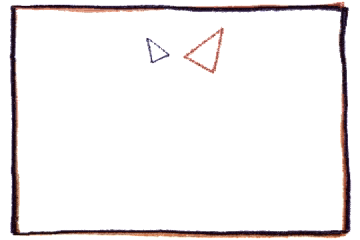
\includegraphics[scale=0.15]{sample65dance.png} & 
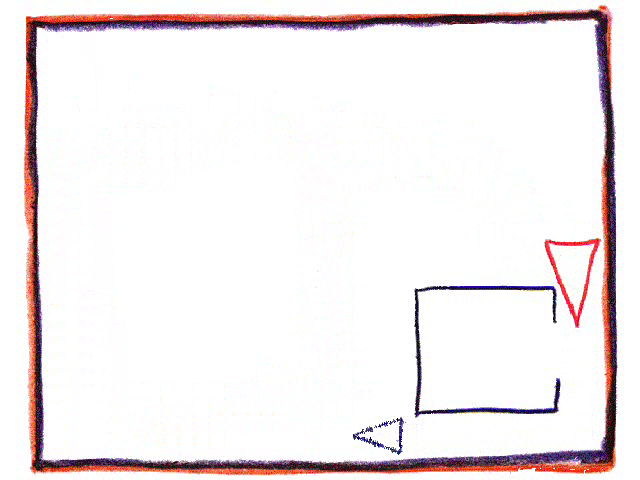
\includegraphics[scale=0.075]{sample174chase.png} &
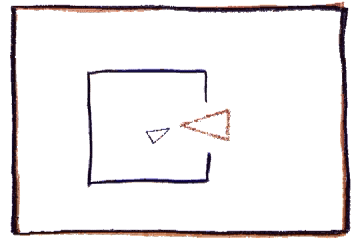
\includegraphics[scale=0.15]{sample198coax.png}
\end{tabular}
\label{tab:gt}
\caption{Stills from animations}
\end{figure}

\section*{Introduction : }  Actions can be based on the the variations in the shape and size change , poses\cite{pami-Ben-ArieWPR02}  or orientation of the object. For example a person walking can be identified by motion of his hands and legs relative to his body. Similar can be said about the actions involving multiple agents. But what if the action which either don't need any shape changes to be expressed or the agent is an abstract object. These type of actions are represented either by specific motion of single object or particular type of motions and interaction between the agents. In this project we analyse the second type of actions. We use psychological videos\cite{fhanimation}. \\

All these videos are goal driven. Most of these animations contain only two agents which are triangles. The videos represent a particular transitive action. We take some of the videos and apply HMM to on the feature vectors extracted from the frames of video. We take frames in small consecutive groups. Then we compare the HMM of each group with  group using mutual acceptance metric. And based on this comparison we create hierarchical clustering of the frames of a single video.   


\section*{Related Work :}
Activity recognition has been a very much worked upon topic by researchers after $1980$. Most of the work has been done on human activity recognition. E. Tapia \cite{TapiaIL04} have used different censors to collect data from home and based on that, they recognise activities. Vail \cite{VailVL07} have formulated activity recognition problem as temporal classification. They use CRF for recognising activity of robots. After that they compare the results with HMM classification.\\
\hspace*{10pt} Considering of psychological videos, Heider-Simmel Videos \cite{heider} have been major attention for noun, verb recognition and linguistic mapping. Mukerjee and Satish(2008)\cite{satish-mukerjee-2008icdl} have used unsupervised approach to cluster visual events into action classes. According to them, in some visual, the objects in the focus are more likely to be the part of the action happening in the videos. They have used merge neural gas algorithm to cluster the events. But there has been very less work done on activity recognition on psychological videos. 
\section*{Algorithm :} We extract feature vector $F =  \{f_1, f_2, \cdots f_s \}$ of length $s$ from each of the  frame in the video. The feature vector passed to HMM is described in the section of feature extraction. We take feature vectors of $20$ frames at a time and feed it to HMM. Below is the formulation of the HMM.\\
\subsection*{Hidden Markov Models :}
	Hidden Markov Models dynamic Bayesian Networks. These are very powerful tool for voice, action recognition\cite{Rabiner89atutorial}, parts of speech tagging etc. A HMM is modeled as  - 
	$$\lambda = \{ A, B, \pi \}$$ 
	Where \\
	\hspace*{30pt} $A$ : State transition probability distribution,\\
	\hspace*{30pt} $B$ : Observation symbol probability distribution and \\
	\hspace*{30pt} $\pi$ : Initial probability distribution.\\ 

Here we compute the log likelihood$P(S|\lambda)$ of the data given the HMM. We use the Mixture of gaussians HMM to compute the log likelihood.\\
Now we divide the feature vectors of all the frames into equal sizes of $20$ taken at distance of $10$ frames. And we calculate he log likelihood for each of the set.\\
\subsection*{Hierarchical Clustering :}
Once we have calculated the log likelihood, we create hierarchical clustering of the this data. The each element of data represents $20$ frames in the video.\\
Now we define mutual acceptance of two HMM as the distance between them. Mutual acceptance is mathematically defined as - \\
$$dist(S_1, S_2) = \frac{|logP(S_1|\lambda _ 1)|}{T_1} +\frac{|logP(S_2|\lambda _ 2)|}{T_2} $$
Where\\
\hspace*{30pt} $T_i$ is the length of the sequence $S_i$ which is $20$ here.\\

\begin{figure}[H]
\centering
Based on this metric we create hierarchical clustering of the data obtained from HMM. We use in built matlab function linkage for this type of clustering. The result here is based on 'euclidean' metric and 'ward' merging method. Ward method is inner squared distance method\\
\centering
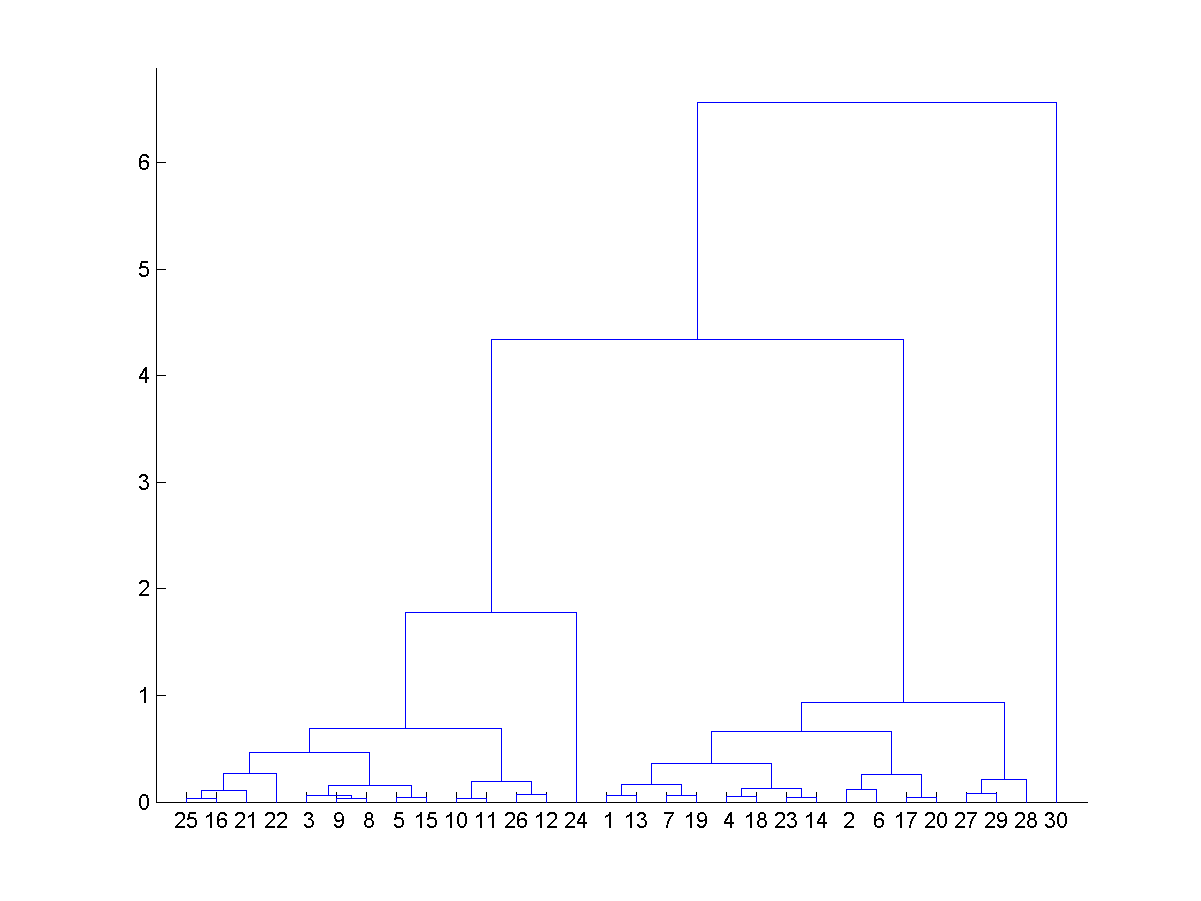
\includegraphics[scale=0.3]{dendoCoax.png}
\caption{Dendrogram plot for coaxing video with  nodes}
\end{figure}

In the hierarchical clustering the data is recursively classified into increasing number of clusters. And thus a hierarchy tree is generated. The leafs represent the individual points in the dataset and the rest of the nodes represent cluster of these points.  The points merging at close to leaf nodes are more similar compared to those merging relatively near the root of the tree. So in our dataset the nodes near the leaves represent the set of frames which are more similar is some way than those in other nodes.
The root of the tree contains all the points in the data. Therefore it represents all the frames of the video. The benefit of hierarchical clustering is that to classify the data in any number or cluster, we need only to cut the tree at appropriate height.\\

\section*{Preprocessing of Data and Feature Extraction : }
We selected $4$ of the videos namely Coaxing, Chase, Mocking, Fighting to use in our project. In the Chase and coaxing video there were three objects, a red triangle, a relatively smaller blue triangle and and a rectangular box. In the rest of the two videos the rectangular box is absent.\\
The frames are converted to gray scale and following steps are done :\\
{\bf Determination of triangles : }\\ \hspace*{10pt} In the first step, we determine the two triangles in the video and track them. To do so one frame of the video is taken as the base frame $frame_0$ and for all the images we calculate the difference of frames :
	$$difference_i = frame_i - frame_0$$
\begin{figure}[H]
\center
\begin{tabular}{cc}
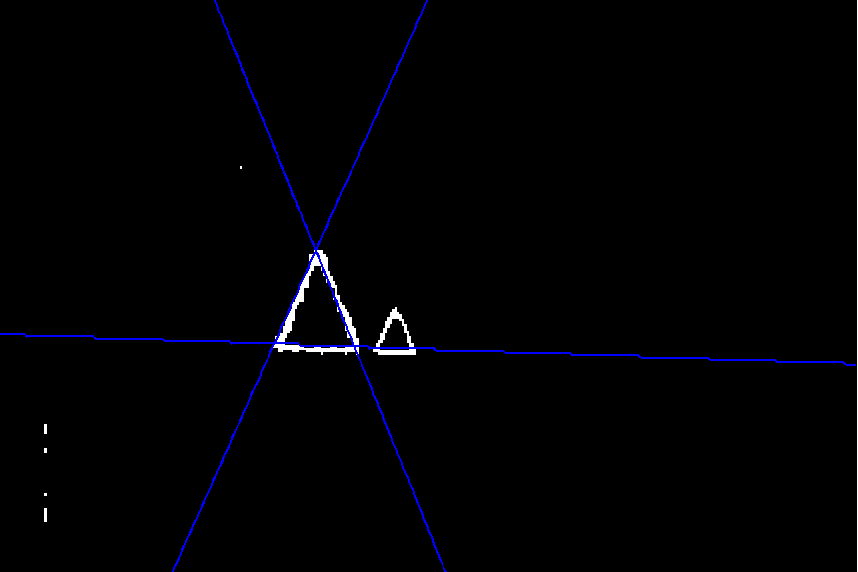
\includegraphics[scale=0.25]{0002l.png} & 
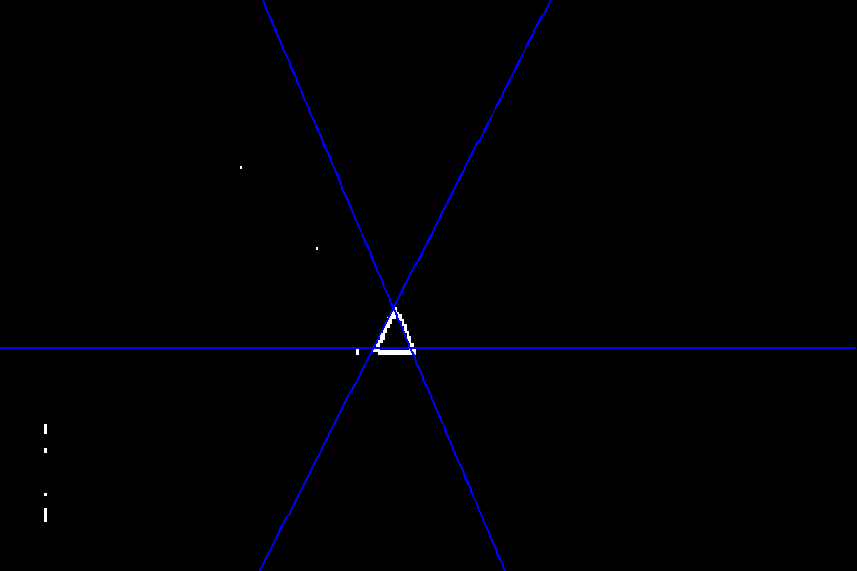
\includegraphics[scale=0.25]{0002s.png}
\end{tabular}
\label{tab:gt}
\caption{Two triangles as detected by Hough Transform}
\end{figure}
Then we apply erosion and dilation to remove the noise in the image. After that Hough transform is applied once on the image to detect the edges of the larger triangle and then on the remaining image to detect the edges of the smaller triangle. Once the edges are determined, centroid if each triangle is calculated.\\
\begin{figure}[H]
{\bf Determination of rectangular box :} \\
 \hspace*{10pt} For the frames which contain the rectangular box, we detect the all sides by Hough Transform based on those, calculate the four vertices of the rectangle. We use midpoint approximation to determine the coordinates of the opening points of the triangles. 
\center
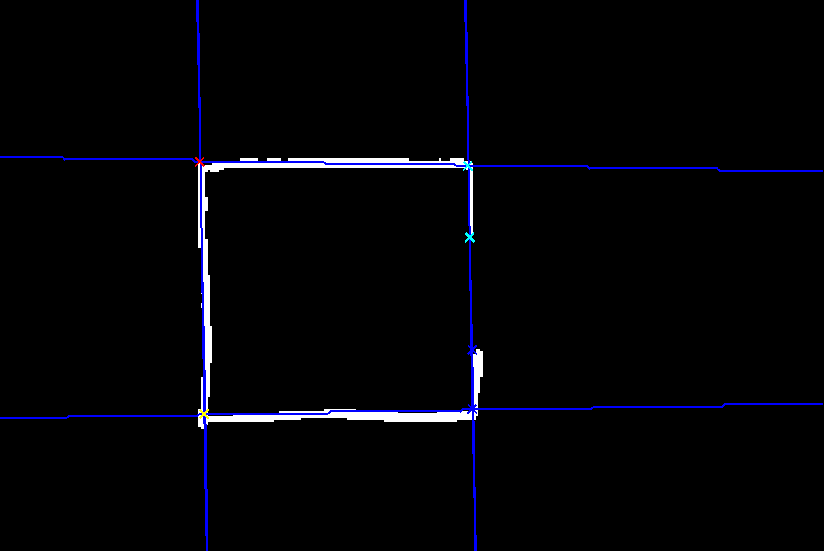
\includegraphics[scale=0.3]{rectCoax.png}
\caption{Vertices of the rectangle detected by Hough Transform}
\end{figure}

\subsection*{Feature Extraction :}
\hspace*{10pt} Since in all these videos an action is represented by the motion of the triangles as well as the interaction between the triangle, we need to know the absolute position and absolute orientation of both the triangles. Apart from that the videos in which the rectangular box is present, it has a lot effect on the action representation of the triangles. Therefore there should be a parameter representing presence of the box in between the triangle. We use visibility of triangles $[0$ $1]$ as the measure of this factor.

\begin{figure}[H]
\hspace*{10pt}
{\bf Orientation of the triangles :}\\
\hspace*{20pt}To determine the orientation of the triangle, we calculate the direction of motion of the triangle. The relative position of the vertex lying around the direction of the motion with respect to the centroid of the triangle will be the orientation of the triangle\\ 
\center
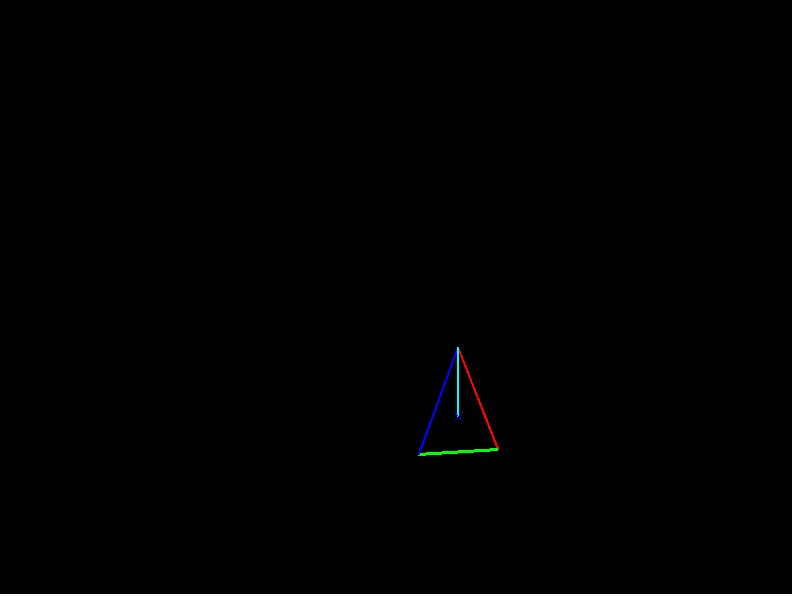
\includegraphics[scale=0.3]{orientation.png}
\caption{Orientation of triangle represented by the cyan line}
\end{figure}

{\bf Visibility of triangles : }\\
\hspace*{20pt}This feature is added to the feature vector only if the rectangle is present in the video. The value of measure of visibility ranges from $0$ to $1$. Visibility of the triangles is calculated by calculating the fraction of the distance between the the supporting lines of the triangles which is hindered by the rectangle. \\
\begin{figure}[H]
\centering
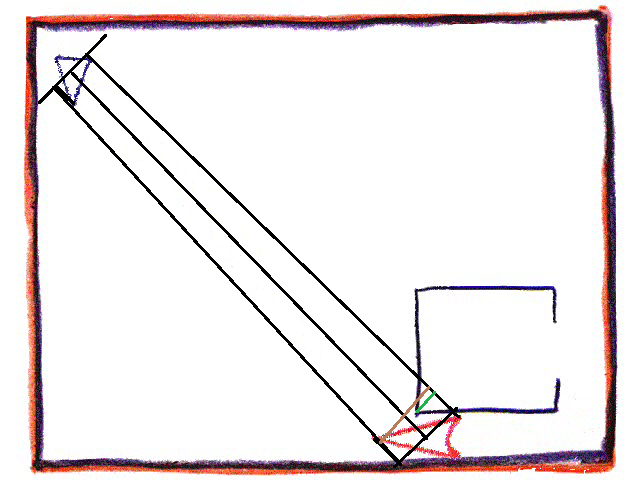
\includegraphics[scale=0.3]{visibility.png}
\caption{The ratio of length of green and brown light is the measure of visibility of the triangles}
\end{figure}
we pass the feature vector consisting of coordinates of the centroids of the triangles, their orientation vector and the visibility of the triangles in the videos where the rectangle is present. So for each frame in the videos containing rectangle, the length of the feature vector is $7$ while those not containing the rectangle have feature vector of length $6$. The results shown here do not use visibility feature.
\section*{Database :}
In this project we have used the animations\cite{fhanimation} created at University of cognitive Neuroscience, UK. These animations were created to study autism in human. Autism creates Theory of Mind deficiency in children and in adults. People suffering from this are not able to predict the actions and thoughts of the other people or objects or in other way they are not able to make a theory about the reaction or interpretation of their surroundings. Traditionally autism was tested by false-belief test. False belief is an attribute in human, which makes them able to believe that other people in world can have different belief than him about same phenomena. This quality is developed in the childhood. But adults with autism were able to pass the false-belief test.\\
\hspace*{10pt} These animations named Frith-Happe animations had better success in capturing autism in adults. There are three major classes of animations. "Random" ,"Goal-Desired", and "Theory of Mind". Each class is made to test different psychological aspect of mind. Each of these class have $4$ videos in it.\\
\begin{figure}[H]
\begin{tabular}{ccc}
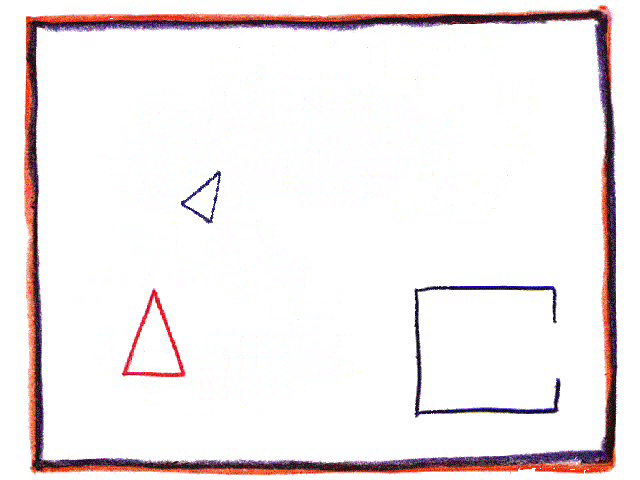
\includegraphics[scale=0.09]{chase348.png} &
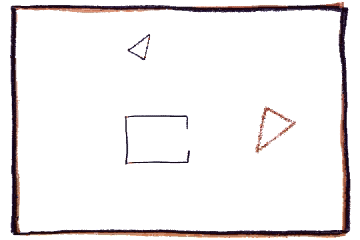
\includegraphics[scale=0.18]{drift271.png} &
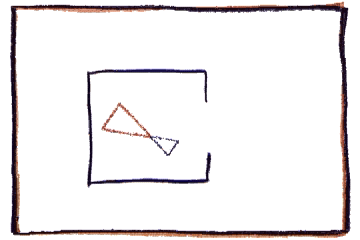
\includegraphics[scale=0.18]{coax88.png}
\end{tabular}    
\label{tab:gt}
\caption{Stills from videos. The leftmost image is from chase video which is in Goal-Directed category, second one is from Drifting which is in random category and third one is from Coaxing video, which is in Theory of Mind Category}
\end{figure}
We used these videos because these videos represent intentionality in them. Generate such video automatically with those is a very difficult problem.
\section*{Commentaries: } We recorded commentaries on two videos Chasing and Coaxing from two different users. The process of recording the commentaries was as follows:-\\
\hspace*{10pt} These two videos were shown to the user 2-3 times and then each user was given certain instruction about the content type of the commentaries. Then the commentaries were taken. Further these commentaries are time-stamped according to the videos. These commentaries will be used in further works on this topic.
\section*{Results :} In the hierarchical clustering obtained, we created tool to visualize the image sets contained in each of the node. By analysing those nodes of the tree, we found that the nodes merging at the lowest level were very similar. Here are the  sample nodes merging  in coaxing videos :-\\

\begin{figure}[H]
\centering
\begin{tabular}{ccc}
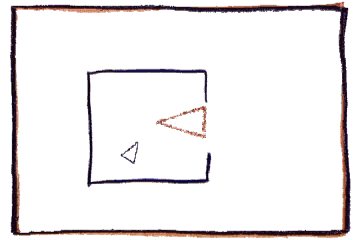
\includegraphics[scale=0.18]{coax210.png} &
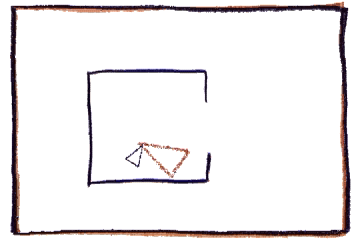
\includegraphics[scale=0.18]{coax220.png} &
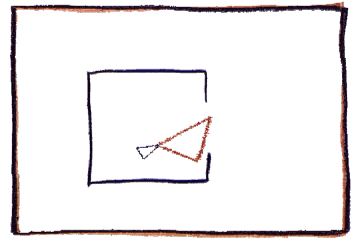
\includegraphics[scale=0.18]{coax240.png} 
\end{tabular}
\caption{Here the first and 2nd image are merged at the first level and on the next level this cluster merges with 3rd image to form another cluster}
\end{figure}


Below are the dendrograms plots of some videos. In each of the dendrogram only merging of $30$ nodes is displayed :\\
First using the acceptance metric and 'ward' merging method the results were - \\

\begin{figure}[H]
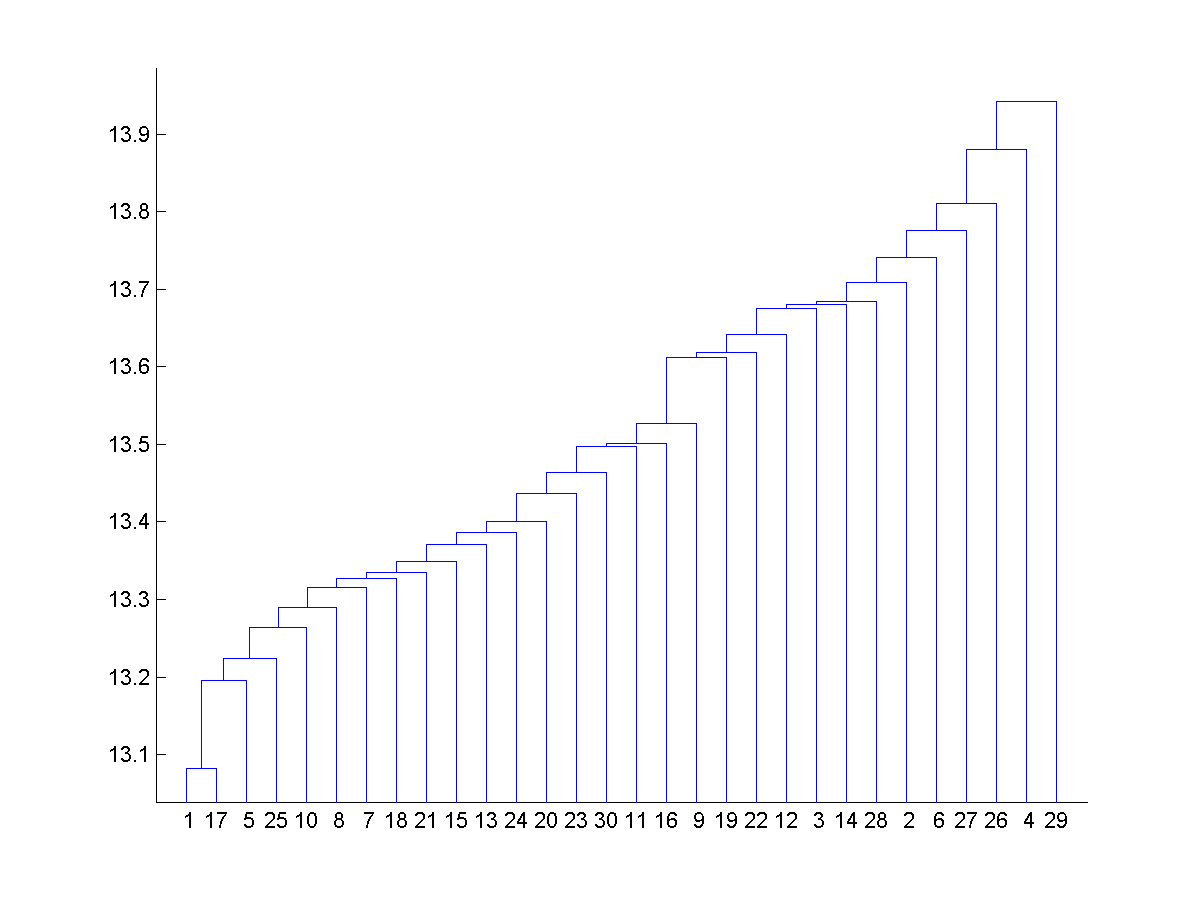
\includegraphics[scale=0.3]{dendo_distance_coax.png}
\end{figure}
\begin{figure}[H]
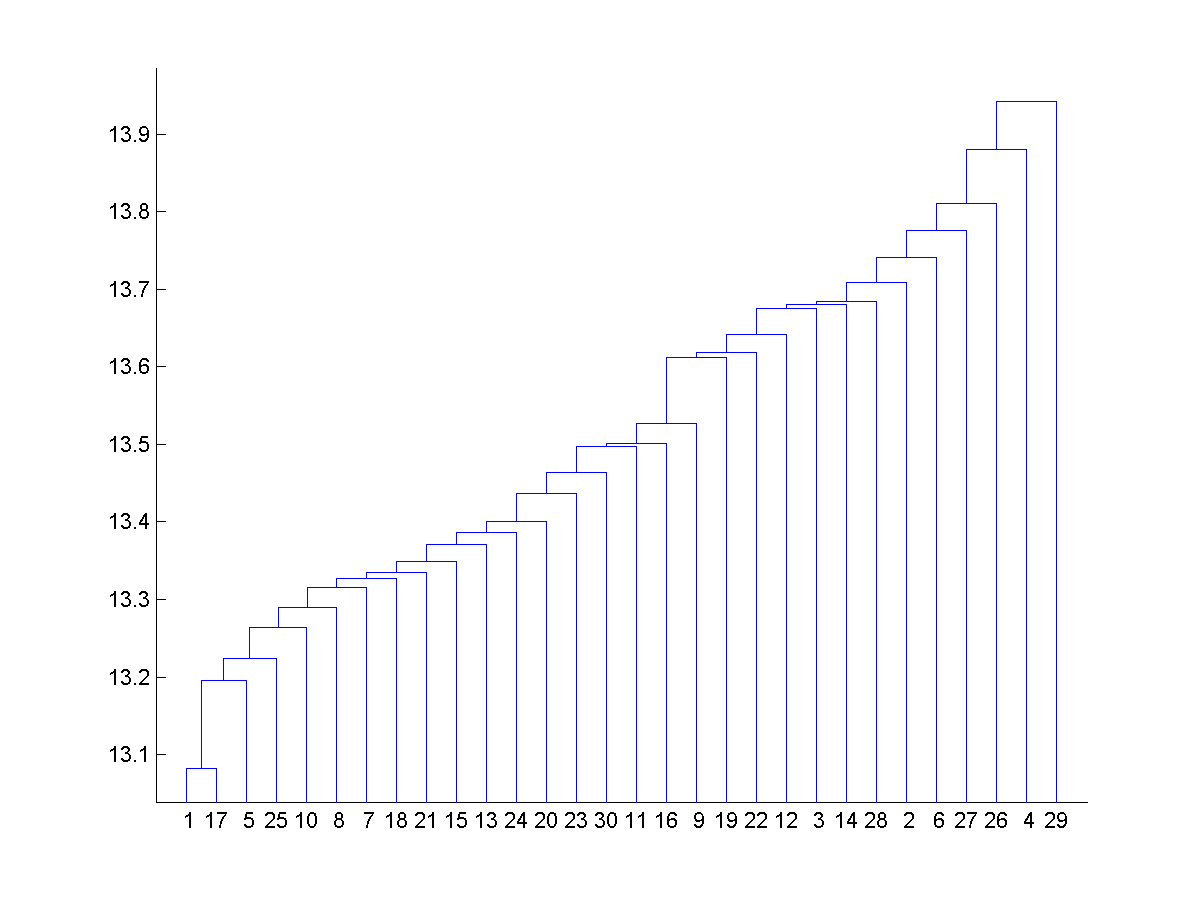
\includegraphics[scale=0.3]{dendo_distance_coax.png}
\caption{The dendrogram plot of the hierarchical clustering mutual acceptance and 'ward' merging}
\end{figure}
Similar results were for other metric and merging methods. The best result was found with 'ward' merging and 'euclidean' distance metric which was as follows :-
\begin{figure}[H]
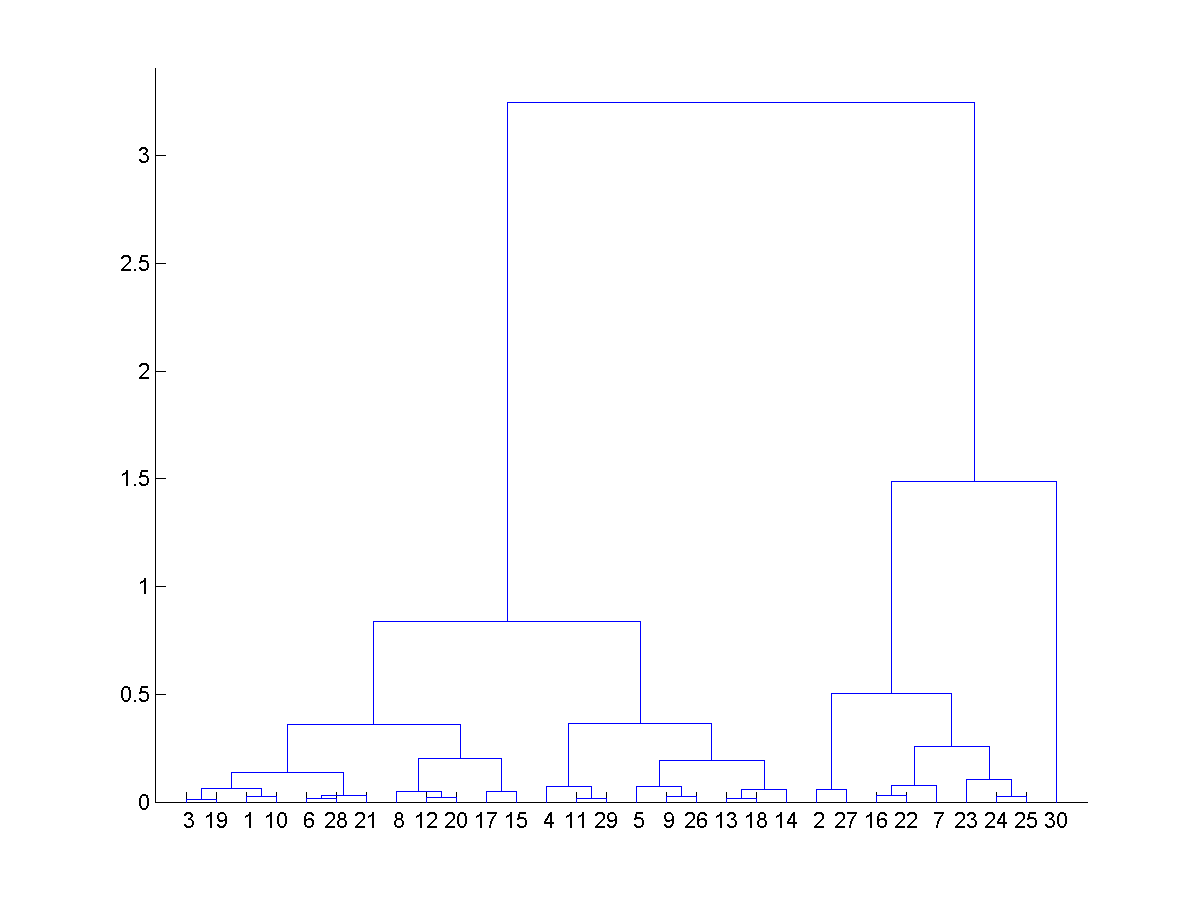
\includegraphics[scale=0.3]{dendoChase.png} 
\begin{figure}[H]
\end{figure}
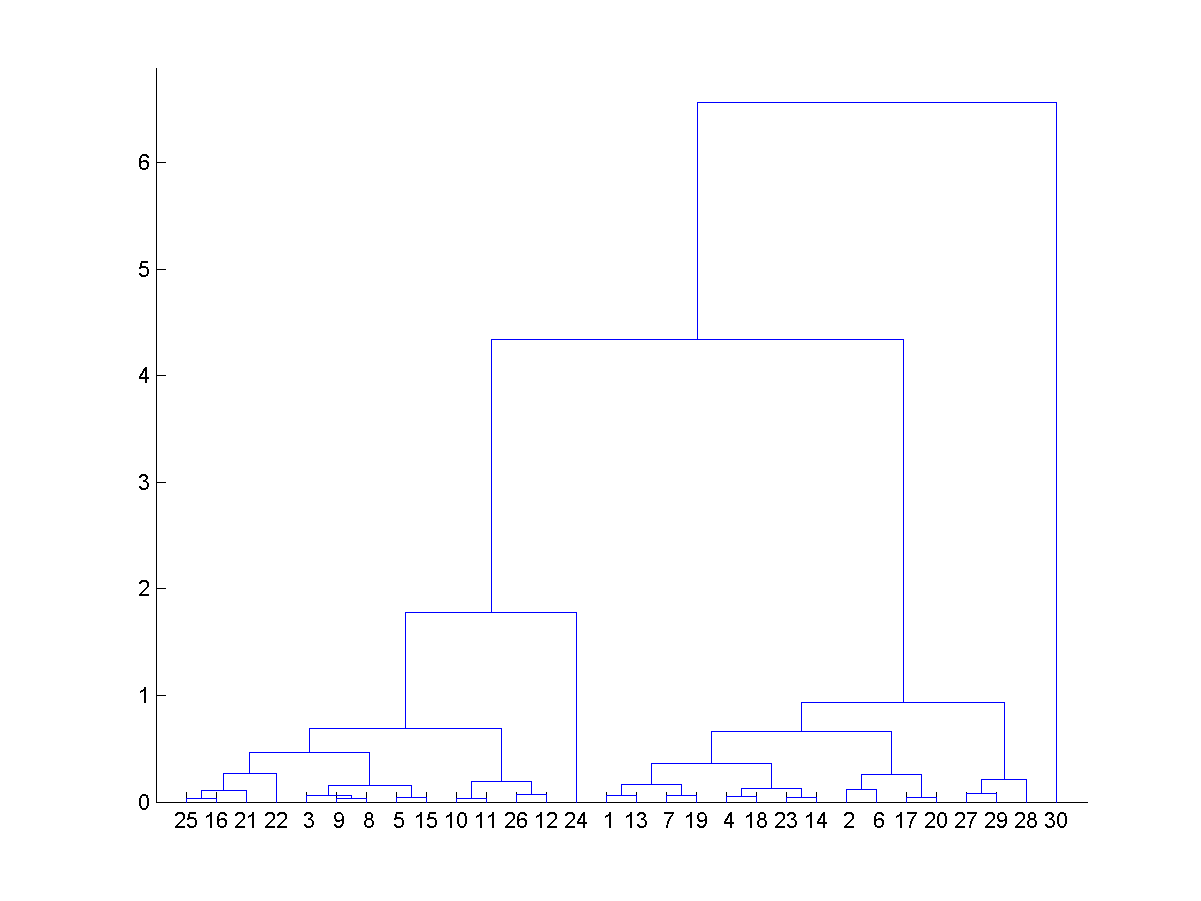
\includegraphics[scale=0.3]{dendoCoax.png}
\caption{The dendrogram plot of the hierarchical clustering with 30 nodes visible}
\end{figure}
\section*{Conclusion and Further Work:}
By hierarchical clustering we get information about which set of frames are more similar to each other and which are less similar. If we take a few of levels from top, these nodes represent one specific kind of interaction or motion of objects. Therefore in the next step we use the commentaries on the same videos and try to find linguistics assigned to the activities represented by the triangles.
\bibliographystyle{plain}
\bibliography{authorName}

\end{document}